\documentclass{article}

% Deactivate sectsty warning when loading sectsty {{{
\usepackage[immediate]{silence}
\WarningFilter[temp]{latex}{Command}
\usepackage{sectsty}
    \sectionfont{\normalfont\sffamily\bfseries\color{blue!40!black}}
    \subsectionfont{\normalfont\sffamily\bfseries\color{blue!30!black}}
\DeactivateWarningFilters[temp]
\makeatletter % disable the runtime redefinitions
\let\SS@makeulinesect\relax
\let\SS@makeulinepartchap\relax
\makeatother
% }}}

\usepackage[margin=3.8cm]{geometry}
    \setlength\parindent{0pt}
\usepackage{fancyhdr}
    \pagestyle{fancy}
\usepackage{fontspec}
    \setsansfont{Linux Biolinum O}
\usepackage{polyglossia}
    \setmainlanguage{english}
\usepackage{sectsty}
    \sectionfont{\normalfont\sffamily\bfseries\color{blue!40!black}}
    \subsectionfont{\normalfont\sffamily\bfseries\color{blue!30!black}}
\usepackage{amsmath}
\usepackage{amssymb}
\usepackage{siunitx}
\usepackage{float}
\usepackage{booktabs}
\usepackage{subcaption}
\usepackage{graphicx}
\usepackage{xcolor}
\usepackage{listings}
    \lstset{language=C++,
	basicstyle=\footnotesize\ttfamily,
	breaklines=true,
	framextopmargin=50pt,
	frame=bottomline,
	backgroundcolor=\color{white!86!black},
	commentstyle=\color{blue},
	keywordstyle=\color{red},
	stringstyle=\color{orange!80!black}}
\usepackage{tikz}

\title{\textsf{\color{blue!40!black}1 Übung IBN}}
\author{Maurice Donner \and Ise Glade}

\begin{document}

\maketitle

\section*{Aufgabe 1}
\begin{itemize}
\item 
The focused thinking mode takes your thoughts along familiar paths. It helps
solve problems with the help of approaches that are already known.\\
The diffused thinking mode is a more relaxed and free approach. It might be
harder to stick to a certain idea, but that is the whole reason why it might be
effective. Its useful for coming up with new concepts and gives the freedom
a creative solution requires.
\begin{itemize}
    \item[a)] \textbf{Focused Thinking} - Learning Vocabulary is a repetitive
	task, that every person may develop a different technique for, but the
	pattern is always the same.
    \item[b)] \textbf{Diffuse Thinking} - This is where the freedom of thought
	comes in handy. 
    \item[c)] \textbf{Focused Thinking} - To learn a new method
	for calculation, the diffused thinking mode might be beneficial. But
	if training is what is needed, repeating the same method for different
	problems over and over again, seems like the best approach
    \item[d)] \textbf{Both Modes} - This is where both modes come together.
	To really understand everything that is taught in the lecture, one
	needs to switch between modes whenever its necessary, because the lecture
	(for most people anyway) teaches both new concepts, and requires to
	practice programming.
\end{itemize}
\item Salvador Dali and Thomas Edison are supposed to have used the same technique
to enter these Modes. It is said, that they would try to fall asleep with
something in their hand, so that once they barely got to enter their dreams,
they would drop the object, and immediately wake up again. They would then use
the newly found ideas they got in this diffused mode and would sit down at their
desk and start focussing on the new thought patterns. That way, they 
supposedly could quickly come up with new ideas, and start manifesting them
by giving them a framework.
\item
John Cleese describes the two modes as "open" and "closed". They're the
equivalent of "diffuse" and "focused" respectively. The open mode allows for
creativity, and seeing clues in problems that are not yet understood, while
it is bad for decisiveness. Only in the focused mode one can really implement
the ideas and go through with them undistracted.
\item An example for a great discovery made in the open mode is the discovery of
Penicillin. It was likely only discovered because Fleming looked at a dish
that hadn't grown a culture, and instead of disposing of it, because of assuming
that there was something wrong with it, he saw a clue, during that time he was
in the open mode. In the closed mode, one tends to follow things they know,
unaccepting of deviations from their expectations.
\item Alfred Hitchcock was of the opinion, that working under pressure does not lead
to good results, so that whenever their team was arguing about something he
would rapidly change the topic, so that moods would calm down, and become more
relaxed, allowing for that open/diffused thinking.
\end{itemize}
\section*{Aufgabe 2} 
Abstraction describes the process of hiding the underlying complexity
of a problem for the purpose of simplifying it and is used in programming
to help visualise routines or algorithms. Lower levels of abstractions
are generally find the closer one gets to hardware, while higher levels
of abstraction are concerned with the general logic of the software.\\
\textbf{An advantage} of abstraction is to avoid duplicates in code for
software development.
By writing subroutines or concepts, working towards a solution for a given
problem becomes easier, since less time will be spent writing the same code
over and over again while losing control of the big picture.\\
\textbf{A clear disadvantage} is the loss of detail, which can lead
to inefficiencies in software.
\section*{Aufgabe 3} 
There are two possibilities:
\begin{itemize}
    \item cache hit with \( t_c \)
    \item cache miss with \( t _{c} + t _{r }  \)
\end{itemize}
\begin{align*}
    &t _{\text{ave}} = (p _{+} \cdot t _{c} ) +
    \left( (1- p _{+} ) \cdot ( t_c + t_r) \right)\\
    \Rightarrow \ &t _{\text{ave}} = ( p _{+} \cdot t_c ) + ( t_c + t_r - p _{+}
    \cdot t_c - p _{+} \cdot t_r ) \\
    \Rightarrow \ &t _{\text{ave}} = t_c + t_r - p _{+} \cdot t_r 
\end{align*}
\section*{Aufgabe 4} 
Let \( t _{\text{ave}} \leq 5 t_c, \quad t_r = 100 t_c\):
\begin{align*}
    &t_c+t_r - p _{+} * t_r = t _{\text{ave}} \\
    \Rightarrow \ &t_c + 100 t_c - p_+ \cdot t_r \leq 5 t_c \\
    \Rightarrow \ &101 t_c - p_+ \cdot t_r \leq 5 t_c \\
    \Rightarrow \ &p_+ \cdot t_r \geq 101 t_c - 5 t_c \\
    \Rightarrow \ &p_+ \cdot t_r \geq 96 t_c \\
    \Rightarrow \ &p_+ \geq 96 \frac{t_c}{t_r} \\
    \Rightarrow \ &p_+ \geq \frac{96 t_c}{100 t_c} \\
    \Rightarrow \ &p_+ \geq 0.96
\end{align*}
The probability \( p_+ \) has to be larger than 96\%

\section*{Aufgabe 5} 
\begin{table}[H]
    \centering
\begin{tabular}{lccc}
    \toprule
    Name & GPR & MMX & XMM \\ \midrule
    Purpose & General & Int/Word operations & Fl.-Point Operations \\
    Size & 64 Bits & 64 Bits & 128 Bits \\
    \# of Registers on the CPU & 16 & 8 & 16 \\ \midrule
    Total capacity in Bits & 1024 & 512 & 2048 \\
    Total capacity in bytes & 128 & 64 & 256 \\
    \bottomrule
\end{tabular}
\end{table}
That makes a total of \( 128+64+256 = 448 \) bytes, which is small compared
to the 1 GiB RAM (0.0000417 \%).

\section*{Aufgabe 6}
The POSIX API uses abstractions to "hide" the internal funcionality from the
programmer. This is mainly for the purpose of simplification, and can lead to
the program to do a system call unknowingly. Since system calls take time, this
can lead to the program slowing down. However, most times these system calls
have to be performed in order to do the necessary calculations. So it might
be a good idea to keep them to a minimum, but this is usually handled by the
libraries themselves, and a programmer doesn't need to spend too much time
optimising. Coding efficiently however stays beneficial, especially when it
comes to the design of complex programs that need to be run many times
over.

\section*{Aufgabe 7}
All exec() functions replace the current process image with a new one.
The following functions are layered on top of execve.
They can be grouped the following:\\

\textbf{Functions with the "-l" suffix}: \texttt{execl(), execlp(), execle()}\\
The list of arguments available to the executed program must be terminated by
a NULL pointer. By contrast to the 'l' functions, the 'v' functions specify
the command-line arguments of the executed program as a vector.\\
\textbf{Functions with the "-v" suffix}: \texttt{execv(), execvp(), execvpe()}\\
The argument list is represented by an array of pointers. The array of pointers
must be terminated by a NULL pointer.\\
\textbf{Functions with the "-e" suffix}: \texttt{execle(), execvpe()}\\
The environment of the caller is specified via the argument \texttt{envp}.
All other \texttt{exec()} functions (without the -e suffix) take the
environment for the new process image from the external variable
\texttt{environ} in the calling process.\\
\textbf{Functions with the "-p" suffix}: \texttt{execlp(), execvp(), execvpe()}\\
These functions duplicate the actions of the shell in searching for an
executable file if the specified filename does not contain a "/" character.
If it does contain a "/" character, then \texttt{PATH} is ignored, and
the file a the specified pathname is executed.\\
In addition, certain errors are treted specially, for example if permission
is denied for a file (\texttt{EACCES}, will continue searching \texttt{PATH})
or the header of a file isn't
recognized (\texttt{ENOEXEC}, will execute shell with \texttt{/bin/sh}).
All other functions (without the -p suffix) 
take a pathname that identifies the program to be executed

All listed functions and their signature can be found in the following:
\begin{lstlisting}
int execl(const char *pathname, const char *arg, ... ,(char*) NULL):
\end{lstlisting}
\begin{lstlisting}
int execlp(const char *file, const char *arg, ... , (char*) NULL;
\end{lstlisting}
\begin{lstlisting}
int execle(const char *pathname, const char *arg, ... , (char*) NULL, char *const envp[]);
\end{lstlisting}
\begin{lstlisting}
int execv(const char *pathname, char *const argv[]);
\end{lstlisting}
\begin{lstlisting}
int execvp(const char *file, char *const argv[]);
\end{lstlisting}
\begin{lstlisting}
int execve(const char *pathname, char *const argv[], char *const envp[]);
\end{lstlisting}
\begin{lstlisting}
int execvpe(const char *file, char *const argv[], char *const envp[]);
\end{lstlisting}

In the first order, the functions \texttt{execv()} and \texttt{execl()} only
differ in the format of the arguments. They both end up calling the same
underlying system call \texttt{execve()}. In this case, \texttt{execv()} is
solely for convenience: If the number of arguments is fixed, it allows
to avoid creating an array.

\section*{Aufgabe 8}
The function \texttt{fork()} returns the process ID of the child process
in case the fork has worked. If it failed, \texttt{fork()} returns a "-1".\\

\textbf{a.} The program creates 9 processes in total. Assuming the first
\texttt{fork()} call is called \( \text{fork} _{1} () \) etc., the process
tree would look like this:
\begin{figure}[H]
    \centering
    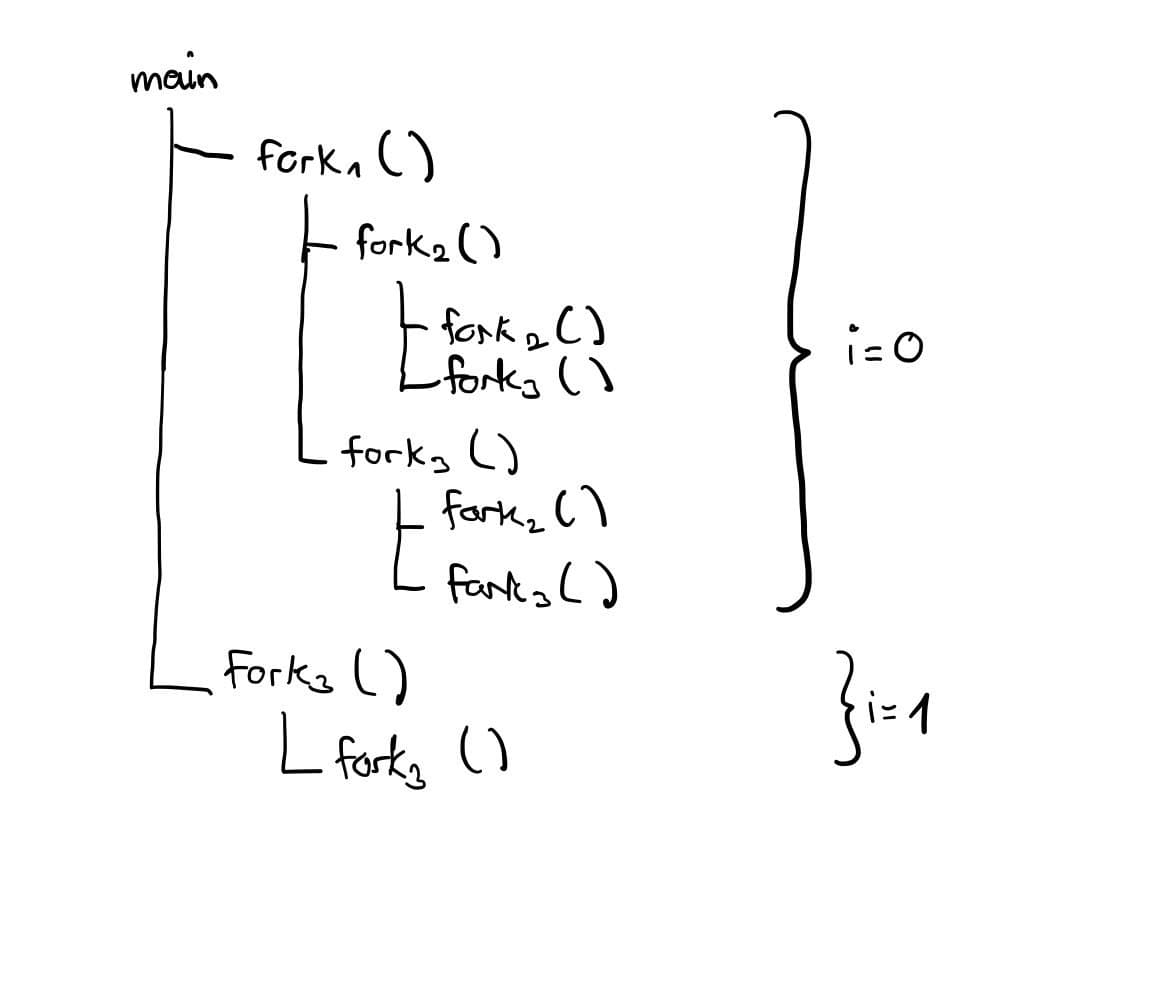
\includegraphics[width=.5\textwidth]{ProcessTree.jpg}
\end{figure}

\textbf{b.} The maximum processes to be started with this program is 11, if 
one assumes the pid of the first fork to be ending on a 1. That means
exactly 10 forks take place, including the parent process, that makes 11.\\
If other processes are started during this process, they might take up
a process id in between, which can increase or reduce the number of forks.

\section*{Aufgabe 9}
\textbf{a)} \texttt{vim}: Software to view and edit text. Everything is
controlled with the keyboard and can run in a single shell. \\
\texttt{cat}: Prints a file on the standard output (the shell), can be
navigated with the scroll wheel. \\

\textbf{b)} Assuming we use vim.
With \texttt{Ctrl-Z} the current job can be stopped. Then the shell can be
used for reading emails (the hardcore vim user might install the ruby-mail
plugin to do this directly in vim aswell). After reading the mail, with
\texttt{jobs}, the job id from the previously stopped job can be seen, and
reopened using \texttt{fg \%[jobid]}. This will get back to where one has
left off.\\

\textbf{c)} With \texttt{cp [file] [destination] \&} copying can be done in 
the background. Then one can get back to reading. In Theory, only 2 processes
are needed for this.One that handles the copying, and one is the program
used to read.

\section*{Aufgabe 10}
During the era of punch cards, writing and compiling code was very slow.
Programmers had to really make sure their program works before testing, as
the testing procedure would cost them lots of time. It was usually faster to
debug the code by hand, instead of compiling it over and over again.\\
Today we use sophisticated error messages and compile programs in the matter
of seconds. We can test subroutines seperately, and use editors, that
will precompile code as we write, showing us where typos might've creeped
in, or declarations might've been forgotten.

\end{document}

